\begin{figure}[ht]
    \centering

    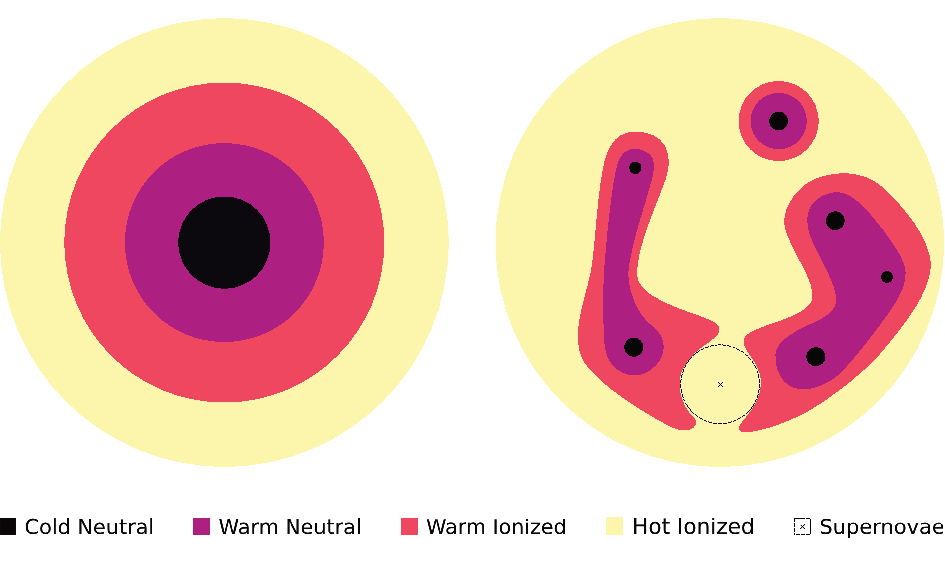
\includegraphics[width=\columnwidth]{structure_v2.pdf}

    \caption{The three-phase structure of the ISM as proposed by \citet{mckee_theory_1977}.
        On the left, the small-scale structure is shown (i.e. one cloud), whereas on the right the large-scale (with multiple clouds) is shown.
        The large-scale picture aims to show the approximate substructure of a single resolution element in the model presented in this work such that an average is taken over this space to produce the subgrid model.
    It should be noted that this figure is for illustration purposes only and does not accurately reflect the relative abundances of the phases; for a more numerical description see \citet{ferriere_interstellar_2001} and the data adapted from it in Table \ref{tab:ism}.}
    \label{fig:struct}
\end{figure}

The study of the substructure of the ISM is important in the development of a subgrid model for within such a model the aim is to take an appropriate `average' over the expected substructure of a given resolution element.
Figure \ref{fig:struct} shows the `standard model' of the structure of the ISM first proposed by \citet{mckee_theory_1977}.
The ISM is made up of three distinct phases, the cold neutral medium, the warm medium, and the hot ionized medium, and these are discussed below.

\subsection{Cold Neutral Phase}

The cold neutral phase of the ISM is the site of star formation; for a recent overview see \citet{mckee_theory_2008} and associated references.
This phase is dense and cold, and is made up of mainly H$_2$ gas, however it is mainly studied observationally by using a close tracer of H$_2$ gas, CO \citep{ferriere_interstellar_2001}.
The H$_2$ gas forms on the surface of dust grains; even though in these regions the density of gas is high relative to the rest of the ISM, the mean free path between two individual hydrogen atoms still remains high.
The dust grains act as a catalyst as the H atoms are adsorbed onto the surface and can react to form H$_2$ more readily there \citep{gould_interstellar_1963}.

Within this region, the gas has almost no thermal pressure support ($v_{rms} < 0.5 \kms$), and so is mainly supported by turbulent motions \citep{larson_turbulence_1981, solomon_mass_1987, heyer_universality_2004} with dispersion $\sigma \approx 1 \kms$.
This dispersion is, however, also small, and as such the gas can coalesce and form stars readily in these regions.
Another important consideration for these regions is that they are shielded from the UV background in the galaxy which is what allows them to reach such cold temperatures; without this shielding the molecular hydrogen would be rapidly dissociated. 

\subsection{Warm Phase}

The warm phase of the ISM is made up of two sub-components: the warm neutral medium and the warm ionized medium, with both phases having a temperature of around $10^4$ K and predominantly being composed of atomic hydrogen.
Above this temperature, the hydrogen can cool radiatively with a high efficiency \citep{gnat_time-dependent_2007}.
The warm neutral medium (see Figure \ref{fig:struct}) is shielded by the warm ionized medium; at the surface of the cloud there is hydrogen constantly being ionized and recombining to re-form neutral hydrogen.
This gas is photoionized by the abundant UV photons in the galaxy that are produced by the O and B stars (\citet{lefloch_photoionization_2001} and associated references).

There appears to be a cut-off in star formation at around 3 scale radii from the galactic centre \citep{kennicutt_star_1989, martin_star_2001}, and it is theorised that this is due to a low column density at those radii \citep{schaye_star_2004}; in those regions the disk is not dense enough to combat the photoionization and collapse to form stars.
From the theoretical predictions outlined in \citep{schaye_star_2004} and observational data from work such as \citet{bigiel_star_2008} (see Figure \ref{fig:bigielwithmart}), the column density at which star formation is viable appears to be in the range of $2.5 - 10 \msun \pc^{-2}$.

\subsection{Hot Phase}

The hot phase of the medium contains ionized hydrogen and highly ionized metals such as O \textsc{vi} and N \textsc{v} which implies a temperature of $10^{5}$ K and above, with the presence of a soft x-ray background at 0.25 keV suggesting regions of $10^6 - 10^7$ K \citep{ferriere_interstellar_2001}.

\subsection{Feedback}

Here it becomes clear that there is a feedback loop; cold gas coalesces to form a cloud, the central region of which can form stars that produce UV photons (and hence a hot phase region).
At the end of the life cycle of these massive clouds, they explode in a supernova, destroying the cloud and injecting energy and turbulence into the ISM.
The ISM can then cool through radiative cooling back to $10^4$ K, self-shield and form a molecular cloud.

\begin{table}[hb]
    \centering
    \resizebox{\textwidth}{!}{
        \begin{tabular}{lccc}
            Phase & $T$ (K) & $\rho$ ($n_H ~\cm^{-3}$)& Observations \\ \hline
            Molecular Gas & $10 - 20$ & $10^2 - 10^6$ & Traced by CO (radio) and IR \\
            Neutral Atomic Gas & $50 - 10000$ & $0.2 - 50$ & Ly$\alpha$ and HI 21 cm radiation \\
            Warm Ionized Gas & $\approx 8000$ & $0.2 - 0.5$ & H$\alpha$ \\
            Hot Ionized Gas & $10^5 - 10^7$ & $10^{-4} - 10^{-2}$ & X-ray and highly ionized metals\\
        \end{tabular}} % end resizebox
    \caption{Overview of the phases of gas in the ISM. Data adapted from \citet{ferriere_interstellar_2001}.}
    \label{tab:ism}
\end{table}
